\subsection{Matrix Multiplication}

The multiplication of matrices is a basic operation in linear algebra and, therefore, a fundamental building block for many scientific applications.
An $n\times d$ matrix $A$ is multiplied with a $d\times m$ matrix $B$ to produce an $n\times m$ matrix $C$, where the elements of $C$ are computed as:
\begin{equation*}
  C_{ij} = \sum_{k=0}^{d} A_{ik} \times B_{kj}, \qquad \forall\ i \in 1, \ldots, n \wedge j \in 1, \ldots, m
\end{equation*}
Here $A_{i*}$ refers to the $i$th row of $A$ and $B_{*j}$ to the $j$th column of $B$.
\autoref{fig:mm} visualizes this computation.
To compute the highlighted element in matrix $C$, the highlighted row of matrix $A$ is combined with the highlighted column of matrix $B$.
For computing the entire matrix $C$, \emph{all pairs} of rows from $A$ and columns of $B$ have to be processed.
Therefore, in \SkelCL the \allpairs skeleton can be used to express matrix multiplication.

\begin{figure}[tb]
  \centering
  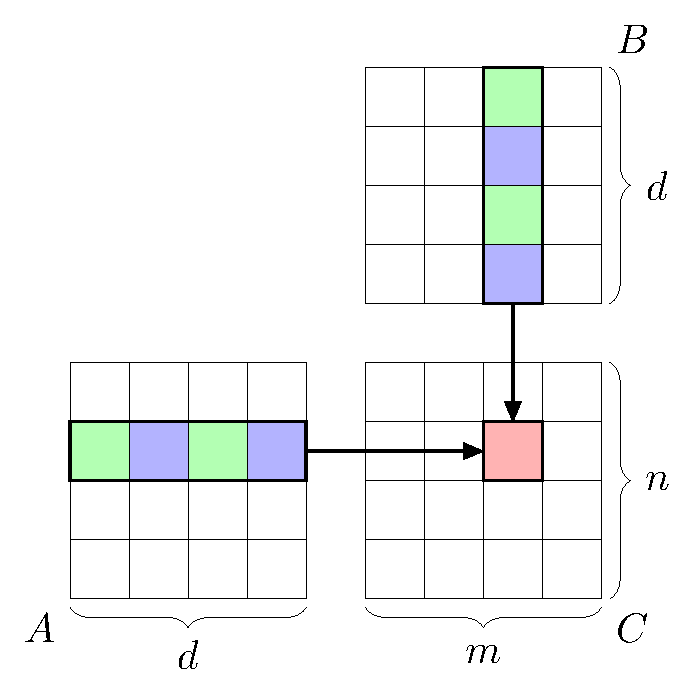
\includegraphics[width=0.5\textwidth]{HLPP/mm}
  \caption[Visalization of matrix multiplication.]%
          {Matrix multiplication $A\times B = C$.
           The red highlighted element in matrix $C$ is computed by combining the highlighted row of matrix $A$ with the highlighted column of matrix $B$.}
  \label{fig:mm}
\end{figure}


\subsubsection*{\SkelCL Implementation}
\autoref{eq:skelcl:mm} shows how matrix multiplication can be expressed using the \allpairs skeleton in \SkelCL:
\begin{align}
  \label{eq:skelcl:mm}
  mm\ A\ B &= allpairs\ f\ A\ B^T\\
  \text{where:} \qquad f\ \vec{a}\ \vec{b} &= \sum_{k=0}^d a_k \times b_k \nonumber
\end{align}
When looking back at \autoref{sec:dot}, we can see, that $f$ is actually the dot product computation, therefore, we can write:
\begin{align}
  mm\ A\ B &= allpairs\ dotProduct\ A\ B^T
  \label{eq:skelcl:mm:dot}
\end{align}
We know that we can express the dot product as a sequential composition of the \zip and \reduce skeletons.
In \autoref{section:skelcl-programming-model:specialSkeletons} we discussed a specialized implementation of the \allpairs skeleton for computations which can be expressed in this way.
Therefore, we can use the \SkelCL library to develop two implementations:
1) using the generic \allpairs skeleton; and 2) using the specialized \allpairs skeleton.

\autoref{lst:skelcl:mm:generic} shows the implementation of matrix multiplication using the generic \allpairs skeleton.
\begin{lstlisting}[%                                                             
caption={Implementation of matrix multiplication using the generic \allpairs skeleton in \SkelCL.},%
numbers=left,%
float=tb,
label={lst:skelcl:mm:generic}]
Matrix<float> mm(const Matrix<float>& A,$\label{lst:skelcl:mm:generic:CPU:start}$
                 const Matrix<float>& B) {
  skelcl::init();
  auto mm = allpairs($\label{lst:skelcl:mm:generic:CPU:stop}$
    [](const Vector<float>& a, const Vector<float>& b) {$\label{lst:skelcl:mm:generic:GPU:start}$
      float c = 0.0f;
      for (int i = 0; i < a.size(); ++i)
        c += a[i] * b[i];
      return c; });$\label{lst:skelcl:mm:generic:GPU:stop}$
  return mm(A, B); }$\label{lst:skelcl:mm:generic:CPU:call}$
\end{lstlisting}
The skeleton is customized with a lambda expression processing two vectors:
$a$ is a row vector of matrix $A$ and $b$ is a column vector of matrix $B$.
In this generic implementation the dot product computation is implemented using a \code{for} loop iterating over the vectors, multiplying elements pairwise and summing them up in the accumulation variable $c$.

\autoref{lst:skelcl:mm:special} shows the implementation of matrix multiplication using the specialized \allpairs skeleton.
\begin{lstlisting}[%                                                             
caption={Implementation of matrix multiplication using the specialized \allpairs skeleton in \SkelCL.},%
float=tb,%                                                                       
numbers=left,%
label={lst:skelcl:mm:special}]
Matrix<float> mm(const Matrix<float>& A,
                 const Matrix<float>& B) {
  skelcl::init();
  auto mult  = zipVector($\label{lst:skelcl:mm:special:zip}$
      [](float x, float y){return x*y;});$\label{lst:skelcl:mm:special:zipGPU}$
  auto sumUp = reduce($\label{lst:skelcl:mm:special:reduce}$
      [](float x, float y){return x+y;}, 0);$\label{lst:skelcl:mm:special:reduceGPU}$
  auto mm    = allpairs(sumUp, mult);
  return mm(A, B); }
\end{lstlisting}
Here the \allpairs skeleton is customized with \zip and \reduce skeletons defined in lines~\ref{lst:skelcl:mm:special:zip} and~\ref{lst:skelcl:mm:special:reduce}.
This implementation corresponds more closely to \autoref{eq:skelcl:mm:dot}:
as we express the dot product using these two skeletons (as shown in \autoref{sec:dot}).
Therefore, we reuse the definitions of \code{mult} and \code{sumUp} as used in \autoref{lst:skelcl:dot}.

\subsubsection*{Implementations used for comparison}
We compare six different implementations of matrix multiplication:
\begin{enumerate}
  \item the OpenCL implementation from~\cite{KirkHw2010} without optimizations,
  \item the optimized OpenCL implementation from~\cite{KirkHw2010} using \GPU local memory,
  \item the optimized BLAS implementation by AMD~\cite{APPML} written in OpenCL,
  \item the optimized BLAS implementation by Nvidia~\cite{cuBLAS} written in CUDA,
  \item the \SkelCL implementation in~\autoref{lst:skelcl:mm:generic} using the generic \allpairs skeleton,
  \item the \SkelCL implementation in~\autoref{lst:skelcl:mm:special} using the specialized \allpairs skeleton.
\end{enumerate}

\paragraph{1. OpenCL implementation}
The kernel of the first, unoptimized OpenCL implementation from~\cite{KirkHw2010} is shown in \autoref{lst:naive_opencl}.
\begin{lstlisting}[%                                                             
caption={[\OpenCL kernel of matrix multiplication without optimizations.]\OpenCL kernel of matrix multiplication without optimizations~\cite{KirkHw2010}.},%
float=tb,%
numbers=left,%
label={lst:naive_opencl}]
kernel void mm(global float* A, global float* B,
               global float* C, int m, int d, int n) {
  int row = get_global_id(0); int col = get_global_id(1);
  float sum = 0.0f;
  for (int k = 0; k < d; k++)
    sum += A[row * d + k] * B[k * n + col];
  C[row * n + col] = sum; }
\end{lstlisting}

\vspace{-.5em}
\paragraph{2. Optimized OpenCL implementations}
The kernel of the optimized OpenCL implementation from~\cite{KirkHw2010} using local memory is shown in \autoref{lst:local_mem_opencl}.
\begin{lstlisting}[%                                                             
caption={[\OpenCL kernel of the optimized matrix multiplication usgin local memory.]\OpenCL kernel of the optimized matrix multiplication using local memory~\cite{KirkHw2010}.},%
float=tb,%
numbers=left,%
label={lst:local_mem_opencl}]
#define T_WIDTH 16
kernel void mm(global float* A, global float* B,
               global float* C, int m, int d, int n) {
  local float Al[T_WIDTH][T_WIDTH];$\label{lst:local_mem_opencl:allocA}$
  local float Bl[T_WIDTH][T_WIDTH];$\label{lst:local_mem_opencl:allocB}$
  int row = get_global_id(0); int col = get_global_id(1);
  int l_row = get_local_id(0);  int l_col = get_local_id(1);
  float sum = 0.0f;
  for (int m = 0; m < d / T_WIDTH; ++m {$\label{lst:local_mem_opencl:loop}$
    Al[l_row][l_col] = A[row * d + (m * T_WIDTH + l_col)];$\label{lst:local_mem_opencl:loadA}$
    Bl[l_row][l_col] = B[(m * T_WIDTH + l_row) * d + col];$\label{lst:local_mem_opencl:loadB}$
    barrier(CLK_LOCAL_MEM_FENCE);$\label{lst:local_mem_opencl:barrier1}$
    for (int k = 0; k < T_WIDTH; k++)
      sum += Al[l_row][k] * Bl[k][l_col];$\label{lst:local_mem_opencl:comp}$
    barrier(CLK_LOCAL_MEM_FENCE); }$\label{lst:local_mem_opencl:barrier2}$
  C[row * n + col] = sum; }
\end{lstlisting}
Two fixed-sized arrays of local memory are allocated in lines~\ref{lst:local_mem_opencl:allocA} and~\ref{lst:local_mem_opencl:allocB}.
Matrix multiplication is carried out in the loop starting in line~\ref{lst:local_mem_opencl:loop}.
In each iteration, data is loaded into the local memory (lines~\ref{lst:local_mem_opencl:loadA} and~\ref{lst:local_mem_opencl:loadB}) before it is used in the computation in line~\ref{lst:local_mem_opencl:comp}.
Note that two synchronization barriers are required (lines~\ref{lst:local_mem_opencl:barrier1} and~\ref{lst:local_mem_opencl:barrier2}) to ensure that the data is fully loaded into the local memory and that the data is not overwritten while other work-items are still using it.

Both OpenCL implementations 1. and 2. from~\cite{KirkHw2010} are restrictive:
they are only capable of performing matrix multiplication for square matrices.

\vspace{-.5em}
\paragraph{3. BLAS implementation by AMD}
The implementation offered by AMD is called clBLAS, written in OpenCL and is part of their Accelerated Parallel Processing Math Libraries (APPML)~\cite{APPML}.

\vspace{-.5em}
\paragraph{4. BLAS implementation by NVIDIA}
The cuBLAS~\cite{cuBLAS} is implemented using CUDA and, therefore, can only be used on GPUs built by NVIDIA.

\subsubsection*{Programming effort}
\autoref{fig:mat_mult_loc} shows the comparison regarding the number of lines of code (LoCs) required for each of the six implementations.
\autoref{tab:mat_mult_loc} presents the detailed numbers.
We did not count those LoCs which are not relevant for parallelization and are similar in all six implementations, like initializing the input matrices with data and checking the result for correctness.
For every implementation, we distinguish between \CPU (host) code and \GPU (kernel) code.

In the \OpenCL implementations, the \GPU code includes the kernel definition, as shown in \autoref{lst:naive_opencl} and \autoref{lst:local_mem_opencl};
the \CPU code includes the initialization of \OpenCL, memory allocations, explicit data transfer operations, and management of the execution of the kernel.

In the BLAS implementations, the \CPU code contains the initialization of the corresponding BLAS library, memory allocations, as well as a library call for performing the matrix multiplication;
no separate definition of \GPU code is necessary, as the \GPU code is defined inside the library function calls.

For the implementation based on the generic \allpairs skeleton (\autoref{lst:skelcl:mm:generic}), we count lines~\ref{lst:skelcl:mm:generic:CPU:start}--\ref{lst:skelcl:mm:generic:CPU:stop} and~\ref{lst:skelcl:mm:generic:CPU:call} as the \CPU code, and the definition of the customizing function in lines~\ref{lst:skelcl:mm:generic:GPU:start}--\ref{lst:skelcl:mm:generic:GPU:stop} as the \GPU code.
For the implementation based on the specialized \allpairs skeleton (\autoref{lst:skelcl:mm:special}), lines~\ref{lst:skelcl:mm:special:zipGPU} and~\ref{lst:skelcl:mm:special:reduceGPU} are the \GPU code, while all other lines constitute the \CPU code.

Both skeleton-based implementations are clearly the shortest, with 10 and 9 LoCs.
The next shortest implementation is the cuBLAS implementation with 65 LoCs -- 7 times longer than the \SkelCL-based implementations.
The other three implementations using \OpenCL require even 9 times more LoCs than the \SkelCL-based implementations.

Besides their length, the \OpenCL-based implementations require the application developer to explicitly implement many low-level, error-prone tasks, like dealing with pointers and offset calculations.
Furthermore, the skeleton-based implementations are more general, as they can be used for arbitrary allpairs computations, while all \OpenCL-based implementations can compute matrix multiplication only.

\begin{figure}[tb]
  \centering
  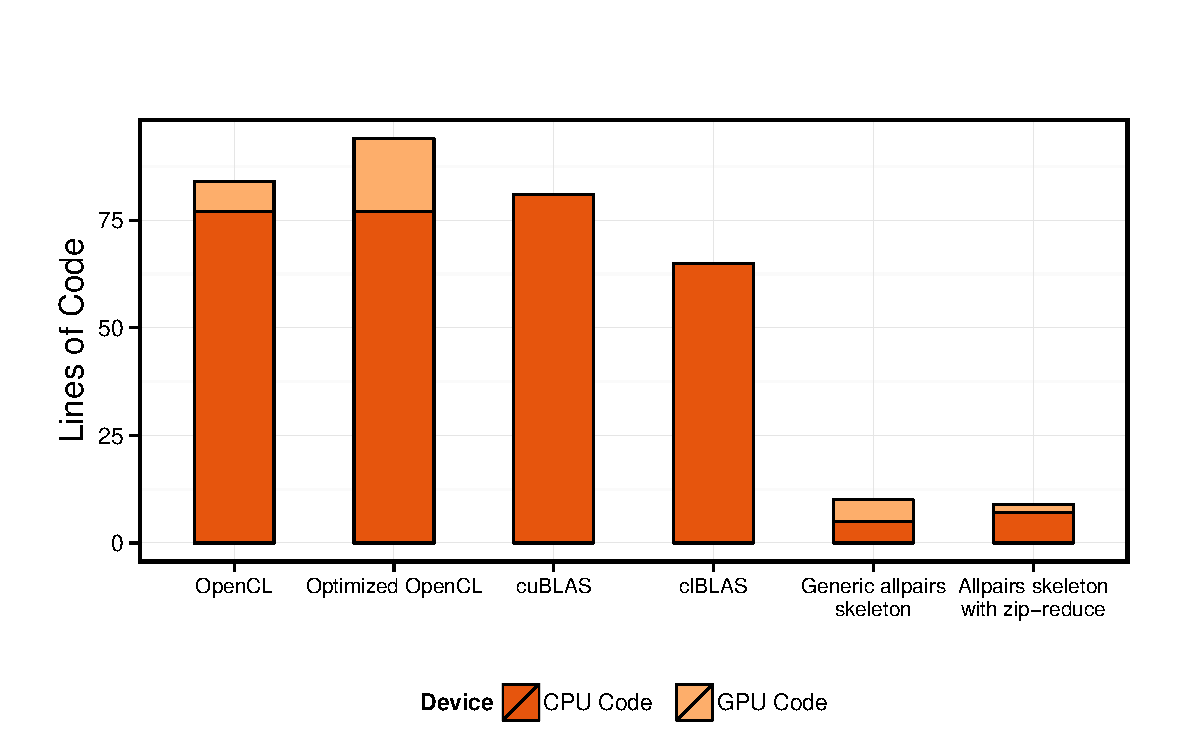
\includegraphics[width=0.9\textwidth]{HLPP/mat_mult_loc}
  \caption[Programming effort of four \OpenCL-based and two \SkelCL-based matrix multiplication implementations.]%
          {Programming effort (Lines of Code) of four \OpenCL-based vs. two \SkelCL-based implementations.}
  \label{fig:mat_mult_loc}
\end{figure}
\begin{table}[tb]
  \centering
  \begin{tabular}{lrr}
    \toprule
              & \multicolumn{2}{c}{Lines of Code} \\
    \cmidrule(r){2-3}
    Implementation & \CPU & \GPU \\
    \midrule
    \OpenCL           & 77 &  7 \\
    Optimized \OpenCL & 71 & 17 \\
    cuBLAS            & 81 & -- \\
    clBLAS            & 65 & -- \\
    Generic \allpairs  & \multirow{2}{*}{5} & \multirow{2}{*}{5}\\
    skeleton\\
    Specialized \allpairs & \multirow{2}{*}{7} & \multirow{2}{*}{2}\\
    skeleton\\
    \bottomrule
  \end{tabular}
  \caption[Lines of Code of matrix multiplication of all compared implementaitons.]%
          {Lines of Code of all compared implementations.}
  \label{tab:mat_mult_loc}
\end{table}

\subsubsection*{Performance experiments}
We performed our experiments with the six different implementations 1. -- 6. of matrix multiplication on two different computer systems with GPUs:
\begin{itemize}[leftmargin=50pt]
  \item[System A:] Our general testing system already described in~\autoref{sec:skelcl:experimental_setup}:
    an NVIDIA S1070 equipped with four Nvidia Tesla \GPUs, each with 240 streaming processors and 4 GByte memory.
  \item[System B:] An AMD Radeon HD 6990 graphics card containing two \GPUs, each with 1536 streaming processors and 1 GByte memory.
\end{itemize}

\begin{figure}[tb]
  \centering
  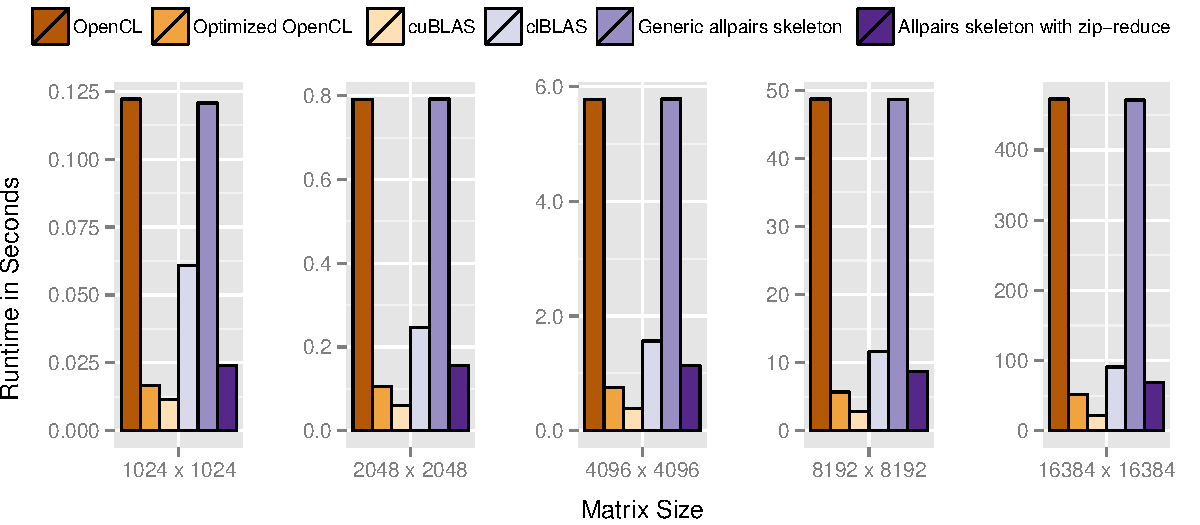
\includegraphics[width=0.9\textwidth]{HLPP/mat_mult_sizes}
  \caption[Runtime of different matrix multiplication implementations on an NVIDIA system.]%
          {Runtime of different matrix multiplication implementations on the NVIDIA system for different sizes of the matrices.}
  \label{fig:mat_mult_single}
\end{figure}
\begin{table}[tb]
  \centering
  \begin{tabular}{lrrrrr}
    \toprule
              & \multicolumn{5}{c}{Runtimes in Seconds} \\
    \cmidrule(r){2-6}
    \multirow{2}{*}{Implementation} & $1024$ & $2048$ & $4096$ & $8192$ & $16384$ \\
                                    & $\times 1024$ & $\times 2048$ & $\times 4096$ & $\times 8192$ & $\times 16384$\\
    \midrule
    \OpenCL            & 0.122 & 0.791 & 5.778 & 48.682 & 472.557 \\
    Optimized \OpenCL  & 0.017 & 0.105 & 0.752 &  5.683 &  51.337 \\
    cuBLAS             & 0.012 & 0.059 & 0.387 &  2.863 &  22.067 \\
    clBLAS             & 0.061 & 0.246 & 1.564 & 11.615 &  90.705 \\
    Generic \allpairs  & \multirow{2}{*}{0.121} & \multirow{2}{*}{0.792} & \multirow{2}{*}{5.782} & \multirow{2}{*}{48.645} & \multirow{2}{*}{471.235} \\
    skeleton\\
    Specialized \allpairs & \multirow{2}{*}{0.024} & \multirow{2}{*}{0.156} & \multirow{2}{*}{1.134} & \multirow{2}{*}{8.742} & \multirow{2}{*}{68.544} \\
    skeleton\\
    \bottomrule
  \end{tabular}
  \caption[Runtime results for all tested implementations of matrix multiplication on an NVIDIA system.]
          {Runtime results for all tested implementations on the NVIDIA system.}
  \label{tab:mat_mult_single}
\end{table}

In all our experiments, we include the time of data transfers to and from the \GPU, \ie the measured runtime consists of:
1) uploading the two input matrices to the \GPU;
2) performing the actual matrix multiplication;
3) downloading the computed result matrix.

\paragraph{System A (one \GPU)}
\autoref{fig:mat_mult_single} shows the runtime in seconds of all six implementations for different sizes of the matrices (note that for readability reasons, all charts are scaled differently).
For detailed numbers, see \autoref{tab:mat_mult_single}.

Clearly, the naive \OpenCL-based implementation and the \SkelCL-based implementation using the generic \allpairs skeleton are the slowest, because both do not use the fast \GPU local memory, in contrast to all other implementations.

The \SkelCL-based implementation using the specialized \allpairs skeleton performs between 5.0 and 6.8 times faster than the implementation using the generic allpairs skeleton, but is 33\% slower on $16384\times 16384$ matrices than the optimized \OpenCL-based implementation using local memory.
However, the latter implementation can only be used for square matrices and, therefore, it benefits from omitting many conditional statements and boundary checks.

\begin{figure}[tb]
  \centering
  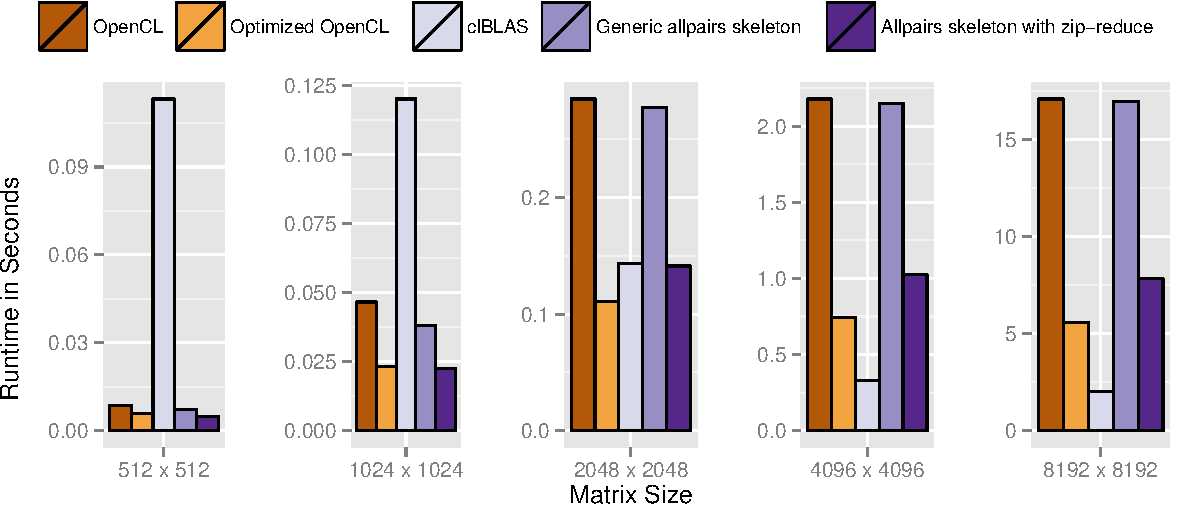
\includegraphics[width=0.9\textwidth]{HLPP/mat_mult_sizes_hd6990}
  \caption[Runtime of different matrix multiplication implementations on an AMD ststem.]%
          {Runtime of all compared implementations for a matrix multiplication on the AMD system using one \GPU.}
  \label{fig:mat_mult_single_amd}
\end{figure}
\begin{table}[b]
  \centering
  \begin{tabular}{lrrrrr}
    \toprule
              & \multicolumn{5}{c}{Runtimes in Seconds} \\
    \cmidrule(r){2-6}
    \multirow{2}{*}{Implementation} & $512$ & $1024$ & $2048$ & $4096$ & $8192$ \\
                                    & $\times 512$ & $\times 1024$ & $\times 2048$ & $\times 4096$ & $\times 8192$ \\
    \midrule
    \OpenCL            & 0.008 & 0.046 & 0.284 & 2.178 & 17.098 \\
    Optimized \OpenCL  & 0.006 & 0.023 & 0.111 & 0.743 &  5.569 \\
    clBLAS             & 0.113 & 0.120 & 0.143 & 0.329 &  2.029 \\
    Generic \allpairs  & \multirow{2}{*}{0.007} & \multirow{2}{*}{0.038} & \multirow{2}{*}{0.278} & \multirow{2}{*}{2.151} & \multirow{2}{*}{16.983} \\
    skeleton\\
    Specialized \allpairs & \multirow{2}{*}{0.005} & \multirow{2}{*}{0.023} & \multirow{2}{*}{0.141} & \multirow{2}{*}{1.025} & \multirow{2}{*}{7.842} \\
    skeleton\\
    \bottomrule
  \end{tabular}
  \caption[Runtime results for all tested implementations of matrix multiplication on an AMD system.]%
          {Runtime results for all tested implementations of matrix multiplication on the AMD system.}
  \label{tab:mat_mult_single_amd}
\end{table}

Not surprisingly, cuBLAS by Nvidia is the fastest of all implementations, as it is highly tuned specifically for Nvidia \GPUs using CUDA.
The clBLAS implementation by AMD using \OpenCL performs not as well:
presumably, it is optimized for AMD \GPUs and performs poorly on other hardware.
Our optimized \allpairs skeleton implementation outperforms the clBLAS implementation for all matrix sizes tested.

\paragraph{System B (one \GPU)}
\autoref{fig:mat_mult_single_amd} shows the measured runtime in seconds for five of the six implementations for different sizes of the matrices.
Detailed numbers can be found in \autoref{tab:mat_mult_single_amd}.
We could not use the Nvidia-specific cuBLAS implementation as it does not work on the AMD \GPU.

For bigger matrices, the slowest implementations are, again, the unoptimized \OpenCL implementation and the implementation using the generic \allpairs skeleton.

The optimized \OpenCL implementation and the specialized \allpairs skeleton perform similarly.
For matrices of size $8192\times 8192$, the optimized \OpenCL implementation is about 30\% faster.

The clBLAS implementation performs very poorly for small matrices, but is clearly the fastest implementation for bigger matrices.
Similar to the cuBLAS implementation on the Nvidia hardware, it is not surprising that the implementation by AMD performs very well on their own hardware.


\begin{figure}[tb]
  \centering
  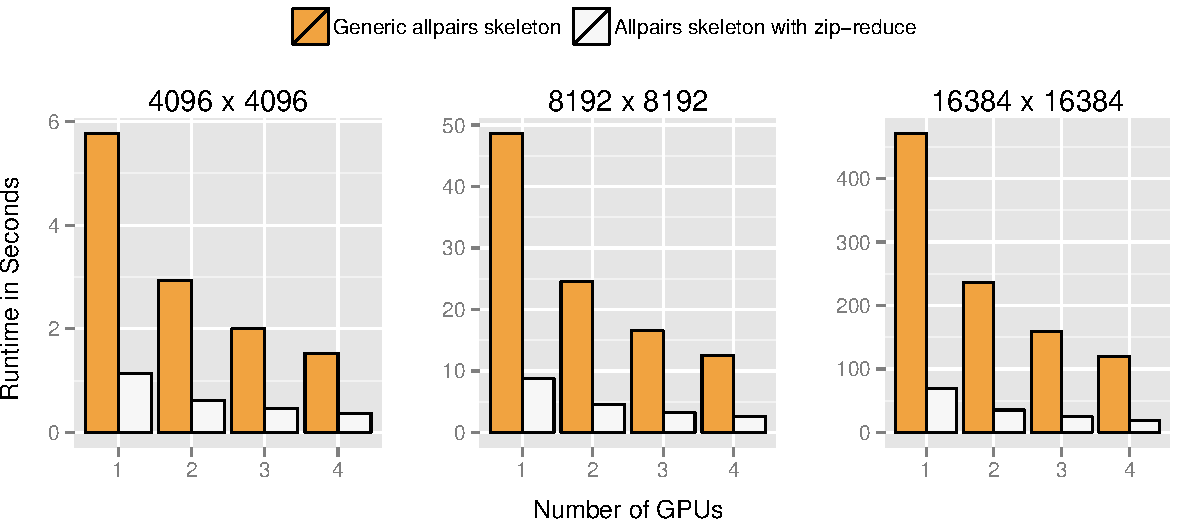
\includegraphics[width=0.9\textwidth]{HLPP/mat_mult_devices}
  \caption[Runtime of the \allpairs based matrix multiplication implementations using multiple \GPUs.]%
          {Runtime of the \allpairs based implementations using multiple \GPUs.}
  \label{fig:mat_mult_devices}
\end{figure}
\begin{table}[tb]
  \centering
  \begin{tabular}{llrrrcr}
    \toprule
              & & \multicolumn{3}{c}{Runtimes in Seconds} & & GFlops\\
    \cmidrule(r){3-5}
    \cmidrule(r){7-7}
    \multirow{2}{*}{Implementation}
     & Number    & $4096$ & $8192$ & $16384$ & & $16384$\\
     & of \GPUs   & $\times 4096$ & $\times 8192$ & $ \times 16384$ & & $ \times 16384$\\
    \midrule
    \multirow{4}{*}{\parbox[t]{2.3cm}{Generic \allpairs\\ skeleton}}
     & 1 \GPU  & 5.772 & 48.645 & 471.328 &&  18.72\\
     & 2 \GPUs & 2.940 & 24.495 & 236.628 &&  37.43\\
     & 3 \GPUs & 2.000 & 16.532 & 158.611 &&  56.17\\
     & 4 \GPUs & 1.527 & 12.540 & 119.786 &&  74.90\\[.5em]
    \multirow{4}{*}{\parbox[t]{2.3cm}{Specialized \allpairs\\ skeleton}}
     & 1 \GPU  & 1.137 &  8.740 &  68.573 && 130.93\\
     & 2 \GPUs & 0.613 &  4.588 &  35.294 && 262.18\\
     & 3 \GPUs & 0.461 &  3.254 &  24.447 && 392.87\\
     & 4 \GPUs & 0.368 &  2.602 &  19.198 && 523.91\\
    \bottomrule
  \end{tabular}
  \caption{Runtime of the allpairs based implementations of matrix multiplication using multiple \GPUs.
    For the matrices of size $16384\times 16384$ the results are also shown in GFlops.}
  \label{tab:mat_mult_devices}
\end{table}

\paragraph{System A (multiple \GPUs)}
\autoref{fig:mat_mult_devices} shows the runtime behavior for both \allpairs skeleton-based implementations when using up to four \GPUs of our multi-\GPU system.
The other four implementations are not able to handle multiple \GPUs and would have to be specially rewritten for such systems.
The newer version of Nvidia's cuBLAS implementation~\cite{} supports the execution on multiple \GPUs as well.
We observe a good scalability for both of our skeleton-based implementations, achieving speedups between 3.09 and 3.93 when using four \GPUs.
Detailed numbers can be found in \autoref{tab:mat_mult_devices}.
For the matrices of size $16384\times 16384$, performance is also provided in GFlops;
to compute this value we excluded the data-transfer time (as usually done in related work) for a better comparison.

\FloatBarrier
